\documentclass[a4paper]{article}
\usepackage{graphicx} 
\usepackage{float} 
\usepackage{subfigure}
\usepackage{amsmath}
\usepackage{indentfirst}
\title{Scientific Computing HW2}
\author{Runze Fang}
\date{\today}

\begin{document}
\maketitle
\section{Solving ill-conditioned linear system}
\subsection{Solving system using the SVD}
I firstly generate a 15 by 15 hilbert matrix $A$ and a right-hand-side so that the exact solution is $x=1$. Then I solve it using the $linsolve$ method.\\
\indent Next, I calculate $\tilde{x}$ by constructing the matrix pseudo-inverse $A^{\dagger}$ from the SVD.\\
\indent Finally, in order to check my constructing method, I test it using a 3 by 3 hilbert matrix and the $pinv$ method. I solve the linear system and compute the relative error in the two approximate solutions $\tilde{x}$. Results are shown below.

\begin{figure}[H] 
\centering 
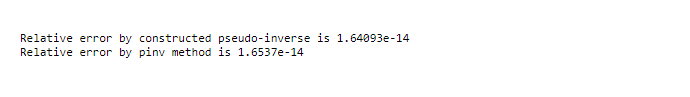
\includegraphics[width=1.0\textwidth]{1.1-1.png}
\caption{test my constructed pseudo-inverse when n=3 hilbert matrix} 
\label{Fig.1.1-1} 
\end{figure}

As shown in the Figure 1, the relative error derived from my construction method is close to the result from $pinv$ method, which indicates my method is a correct way to construct the pseudo-inverse method. Now, I apply my method to the 15 by 15 hilbert matrix. I compute the relative error derived from all three ways: $linsolve$, my own method, and $pinv$. By the way, I compute the P-condition number of my matrix $A$ by dividing the largest eigenvalue of $A$ by the smallest eigenvalue of $A$. $P(A)=|\frac{max\lambda_i}{min\lambda_i}|$ 

\begin{figure}[H] 
\centering 
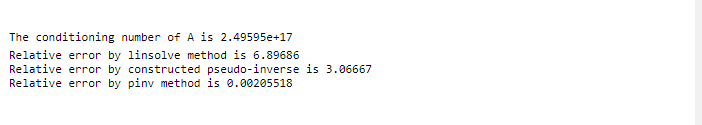
\includegraphics[width=1.0\textwidth]{1.1-2.png}
\caption{conditioning number and relative error in the approximate solution computed in 3 ways} 
\label{Fig.1.1-2} 
\end{figure}

As shown in Figure 2, the P-conditioning number $P(A)=|\frac{max\lambda_i}{min\lambda_i}|=2.49595e17$ , which is extremely large, showing $A$ is extremely ill-conditioned. The relative error from the $linsolve$ approximation is huge. After using $A^{\dagger}$ to do the approximation, the approximate $\tilde{x}$ is more accurate than the direct solution. The relative error becomes a half of the $linsolve$ approximation, but it is around 10 and still not optimal. The approximation using $pinv$ is the most optimal, which has a ralative error of 0.008. This may because the 15 by 15 hilbert matrix has some extreme small singular values which will cause huge roundoff error in computation.

\subsection{Rgularized Pseudo-Inverse}
I generate logarithmically-spaced tolerance $\varepsilon = 10^{i} for i = 1,2...16$. Then I compute the modified pseudo-inverse by setting setting to zero all singular values that are smaller than $\varepsilon\sigma_{1}$ and then get $\tilde{x}$ for each $\varepsilon$. I compute it by my own function and test my result using $pinv$. Then I plot the relative error.

\begin{figure}[H] 
\centering 
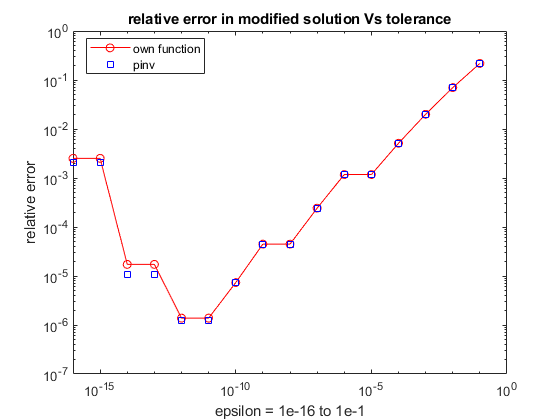
\includegraphics[width=1.0\textwidth]{1.2-1.png}
\caption{relative error in modified solution Vs different tolerance} 
\label{Fig.1.2-1} 
\end{figure}

As shown in the Figure 3, my own function has about the same result as the $pinv$ did. When $\tilde{\varepsilon} \in [10^{-12},10^{-11}]$, we get the smallest relative error $= 1.3815e-06$. 
\subsection{Error Analysis}
When $\epsilon$ is large, we get rid of small singular values. In this case, our computation is accurate, however, we have a large approximation error. Since we get rid of too many singular values, we lost too many features of the matrix. The approximation error dominates the relative error.\\
\indent When $\epsilon$ is small, we keep most of singular values. Small singular values cause huge roundoff error. In this senario, we have small approximation error. However, some singular values are too small to calculate. When we calculate the pseudo-inverse, many reciprocal of singular values are rounded-off to zero. They reached the digit accuracy of matlab. This time, roundoff error dominates the relative error.\\
\indent The statement that "no numerical method can solve an ill-conditioned problem accurately" is still correct, though pseduo-inverse can solve this ill-conditioned linear system. The pseudo-inverse method may lack of universality. Since many ill-conditioned linear systems are unstable only for certain error vectors, pseudo-inverse method may not solve all ill-conditioned problem accurately.

\section{Digraph Matrix of English}
I choose the novel $Harry Potter$ as my text. I read in the text and then construct the digraph matrix $A$ for the text. Then I normalized it and plot it using $imagesc$.

\begin{figure}[H] 
\centering 
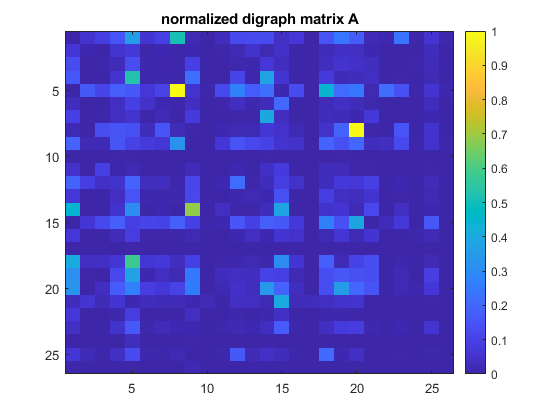
\includegraphics[width=1.0\textwidth]{2.1-1.png}
\caption{normalized digraph matrix} 
\label{Fig.2.1-1} 
\end{figure}

Then I compute the SVD. The following 3 diagram are the rank-1 component, the second principal component and the rank 2 approximation to the matrix.

\begin{figure}[H] 
\centering 
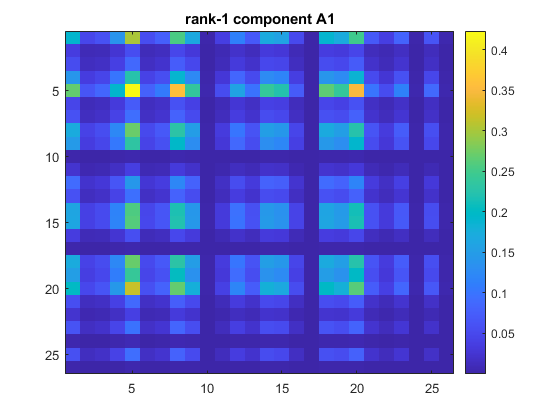
\includegraphics[width=1.0\textwidth]{2.1-2.png}
\caption{rank-1 component} 
\label{Fig.2.1-2} 
\end{figure}

\begin{figure}[H] 
\centering 
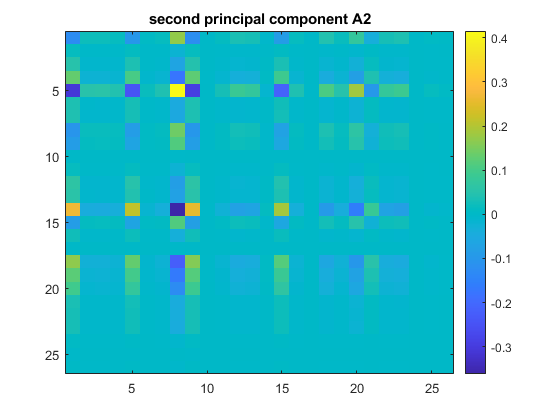
\includegraphics[width=1.0\textwidth]{2.1-3.png}
\caption{second principal component} 
\label{Fig.2.1-3} 
\end{figure}

\begin{figure}[H] 
\centering 
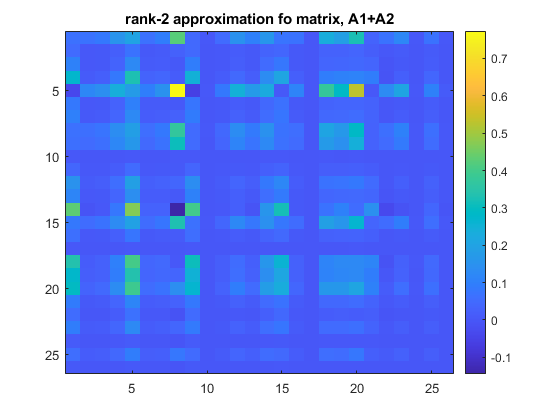
\includegraphics[width=1.0\textwidth]{2.1-4.png}
\caption{rank-2 approximation} 
\label{Fig.Fig.2.1-4} 
\end{figure}

Then I do $sum(A)$ to computes the frequency of occurrence of the different letters.

\begin{figure}[H] 
\centering 
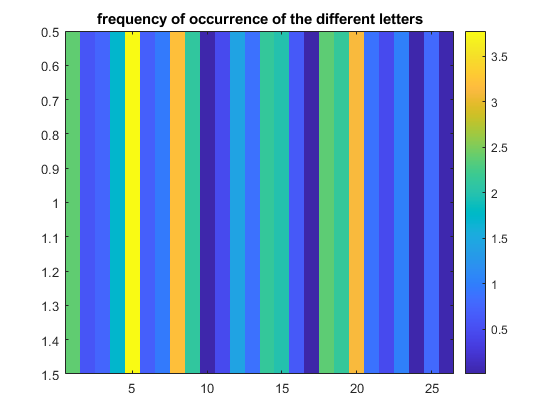
\includegraphics[width=1.0\textwidth]{2.1-5.png}
\caption{frequency of occurence of the different letters} 
\label{Fig.Fig.2.1-5} 
\end{figure}

By observing Figure 5, the rank-1 component, we can see that letter $a$, $e$, $h$, $i$, $r$, $s$, $t$ appears more frequently than other letters since the color in these columns are more yellow than others. Then I do $sum(A)$ to get the frequency of occurrence of the different letters. As shown in Figure 8, we can see clearly the most frequently appearing letter are the $5^{th}$, $8^{th}$ and $20^{th}$ letter, which are letter $e,h,t$. This might be the word $the$ and the word $he$, which are widely used in English. This observation conforms the observation in Figure 4: we can see that the only two yellow are the grid of $he$ and $th$.\\
\indent Then I take a look to the second principal component. I did the permutaion to reorder the letter so that the vowela appears firstly. The figure is shown below.

\begin{figure}[H] 
\centering 
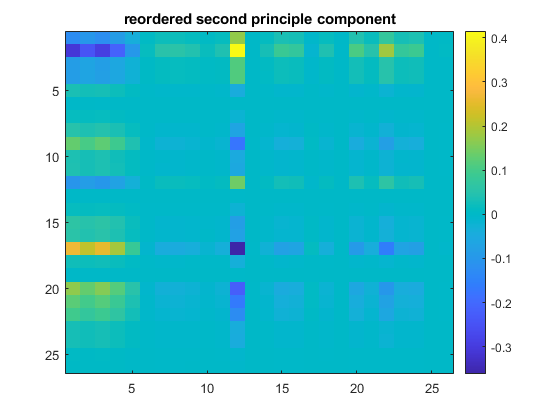
\includegraphics[width=1.0\textwidth]{2.1-6.png}
\caption{reordered second principle component} 
\label{Fig.Fig.2.1-6} 
\end{figure}

As shown in Figure 9, the upper-left corner is relatively blue, which indicates that in English, two consecutive vowels are rarely used. Moreover, the yellow zone appears at the top and left side of the graph. This feature indicates, that a vowel and a consonant combination is the most popular combanation in English. By the way, the $vowel + n$ combination is so popular, for example $an$, $-en$, $in$ and $-on$. \\
\indent Now we compare Figure 4 and Figure 6. We can see that the rank-2 approximation miss the feature that $th$ is one of the most commonly used combination in english.\\
\indent Since the text of $Harry Potter$ is large enough, I try a shorter text to see whether the longitude of text will influence the test result. This time I copy the wiki page of Latex. The normalized digraph, frequency of occurrence of letters and reordered second component graph are shown below.

\begin{figure}[H] 
\centering 
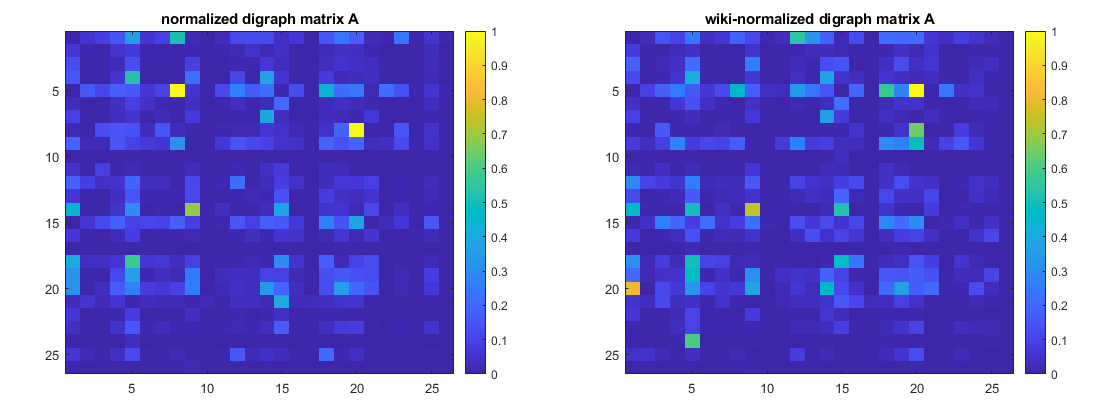
\includegraphics[width=1.0\textwidth]{2.3-1.png}
\caption{normalized digraph: Harry Potter(L) Vs wiki-Latex(R)} 
\label{Fig.2.3-1} 
\end{figure}

\begin{figure}[H] 
\centering 
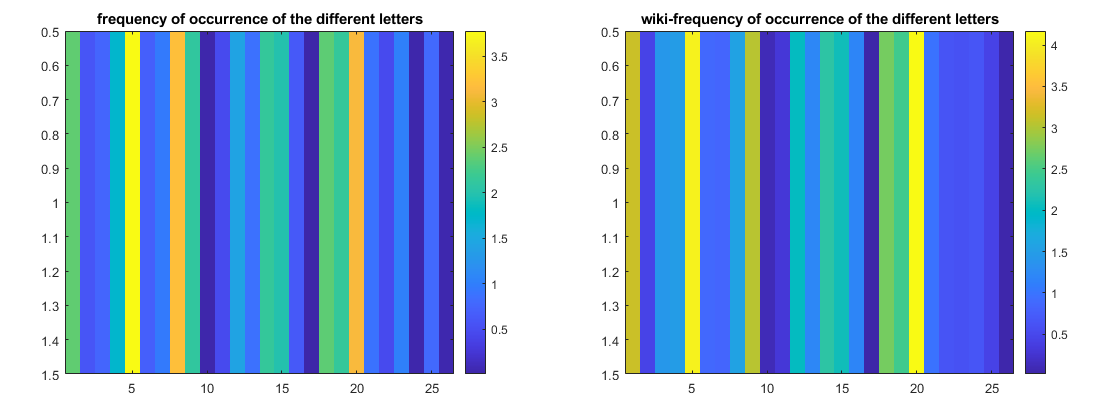
\includegraphics[width=1.0\textwidth]{2.3-2.png}
\caption{frequency of occurrence: Harry Potter(L) Vs wiki-Latex(R)} 
\label{Fig.2.3-2} 
\end{figure}

\begin{figure}[H] 
\centering 
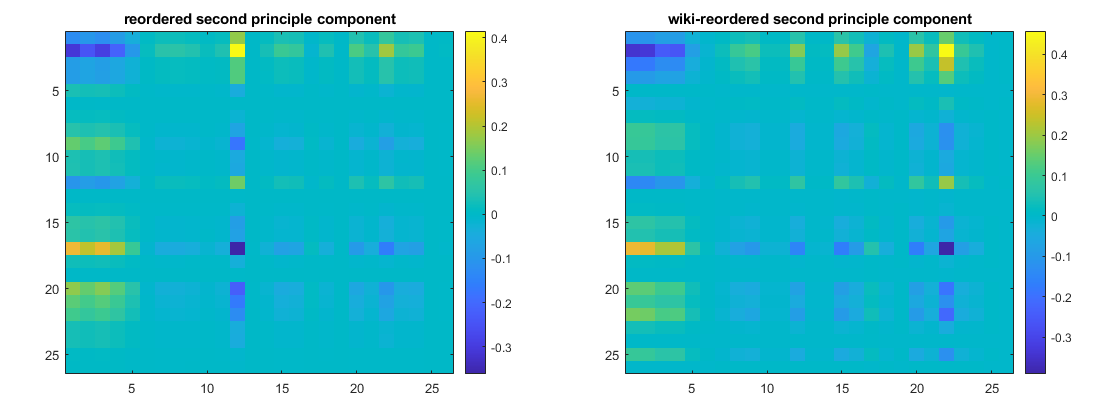
\includegraphics[width=1.0\textwidth]{2.3-3.png}
\caption{reordered second component: Harry Potter(L) Vs wiki-Latex(R)} 
\label{Fig.2.3-3} 
\end{figure}

As shown in Figure 10, the combination $la$, $at$ and $te$ in wiki page of Latex occurs much more than them in $Harry Potter$. This may because of two reason. Firstly, the wiki page is much shorter than $Harry Potter$. Secondly, the topic of the wiki page I have chosen is Latex, therefore, the unusual combination $la$, $at$ and $te$ become more yellow. Same case happens to the frequency of occurence diagram. As shown in Figure 11, the, letter $a$, $t$ and $x$ occurs more frequently in wiki page of Latex, while letter $h$ is obviously less frequent. This is also because the pharse $Latex$, which is seldomly used in common situation, is largely used in the wiki page of Latex. In Figure 12, we can see that the trend of using vowels and consonants is not largely influenced by the longitude of text. In conclusion, the longitude of text does influence the observation of the feature of English. When the text is relatively short and about a specific topic, we will observe features with bias. Although the observation will have some common feature of English, we cannot conclude which feature is the common feature of English.\\
\indent To find out how long the text is needed to be to see the features, I chose the novel $Walden$ and did another test and compared the result with $Harry Potter$. The normalized digraph, frequency of occurrence of letters and reordered second component graph are shown below.

\begin{figure}[H] 
\centering 
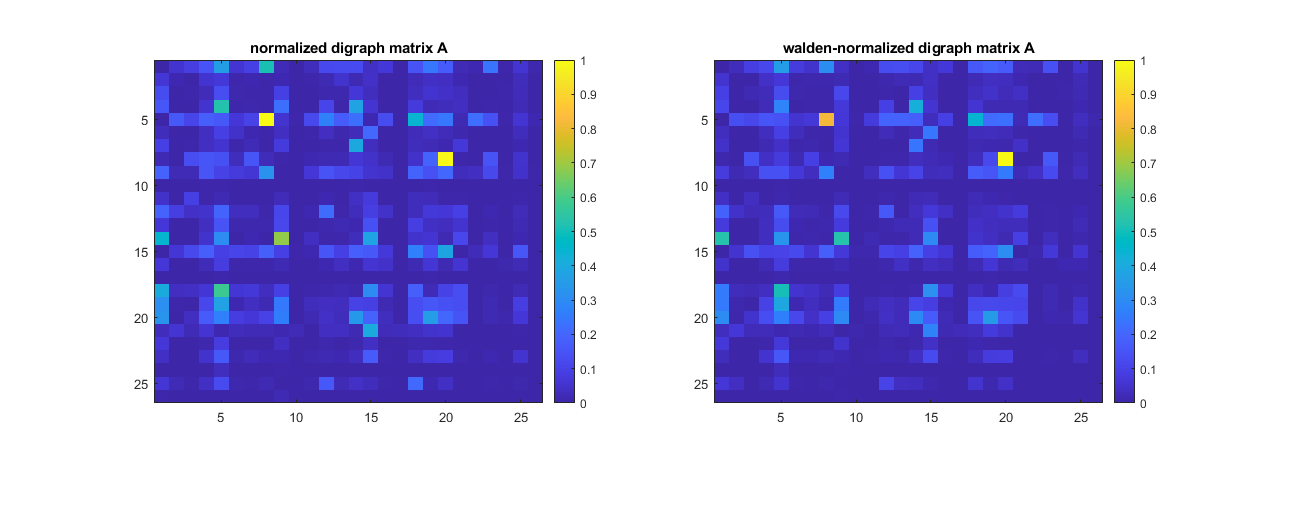
\includegraphics[width=1.0\textwidth]{2.6-1.png}
\caption{normalized digraph: Harry Potter(L) Vs Walden(R)} 
\label{Fig.2.6-1} 
\end{figure}

\begin{figure}[H] 
\centering 
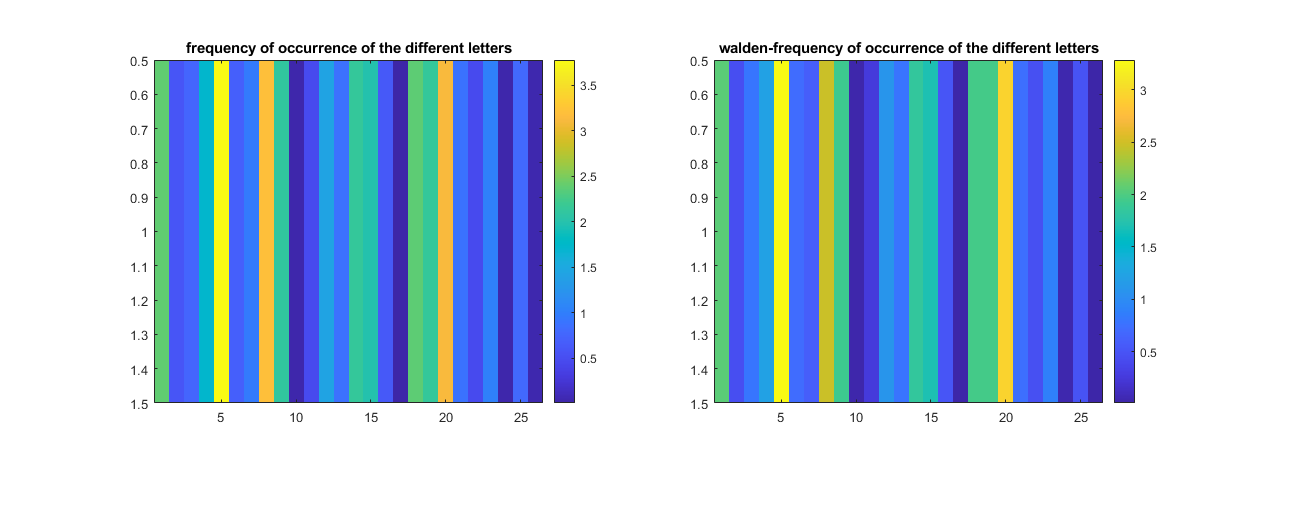
\includegraphics[width=1.0\textwidth]{2.6-2.png}
\caption{normalized digraph: Harry Potter(L) Vs Walden(R)} 
\label{Fig.2.6-2} 
\end{figure}

\begin{figure}[H] 
\centering 
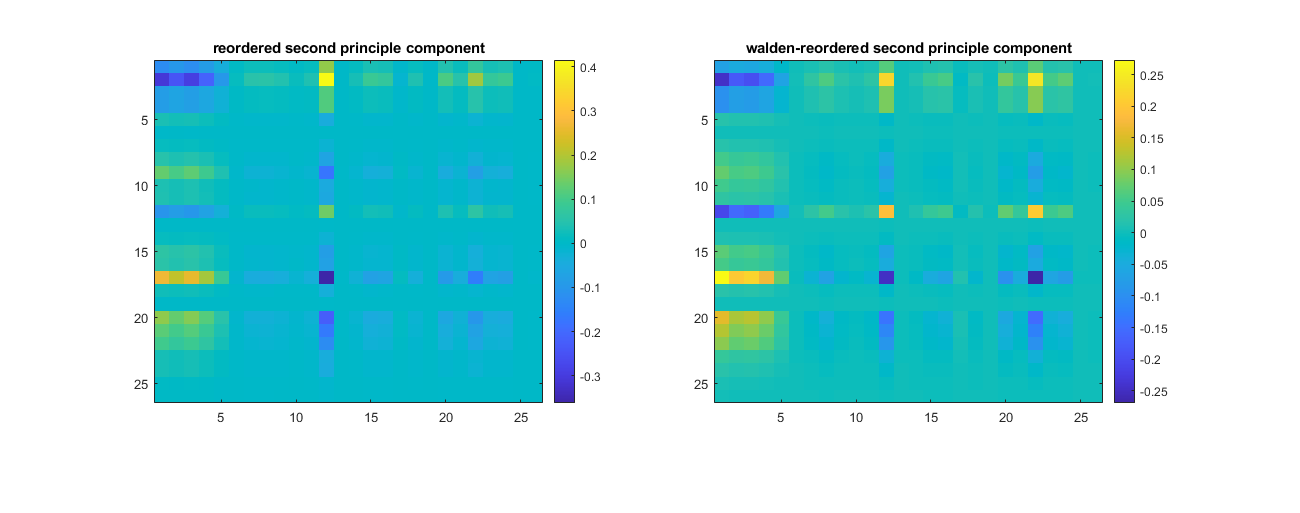
\includegraphics[width=1.0\textwidth]{2.6-3.png}
\caption{normalized digraph: Harry Potter(L) Vs Walden(R)} 
\label{Fig.2.6-3} 
\end{figure}

As shown in Figure 13, Figure 14 and Figure 15, we can conclude the same feature from testing result of $Harry Potter$ and $Walden$: common pattern of $th$ and $he$ and special combination rules of vowels and consonants. Although they have slightly different in some region: some yellow grid may be ligher or some blue grid may be darker, the whole trend is the same. Therefore, from my perspective, the tesxt sample should be at least novel-long to make sure we can get the common feature of English.

\end{document}